\section{Implementation}
\begin{minipage}{1.0\columnwidth}
    \centering
    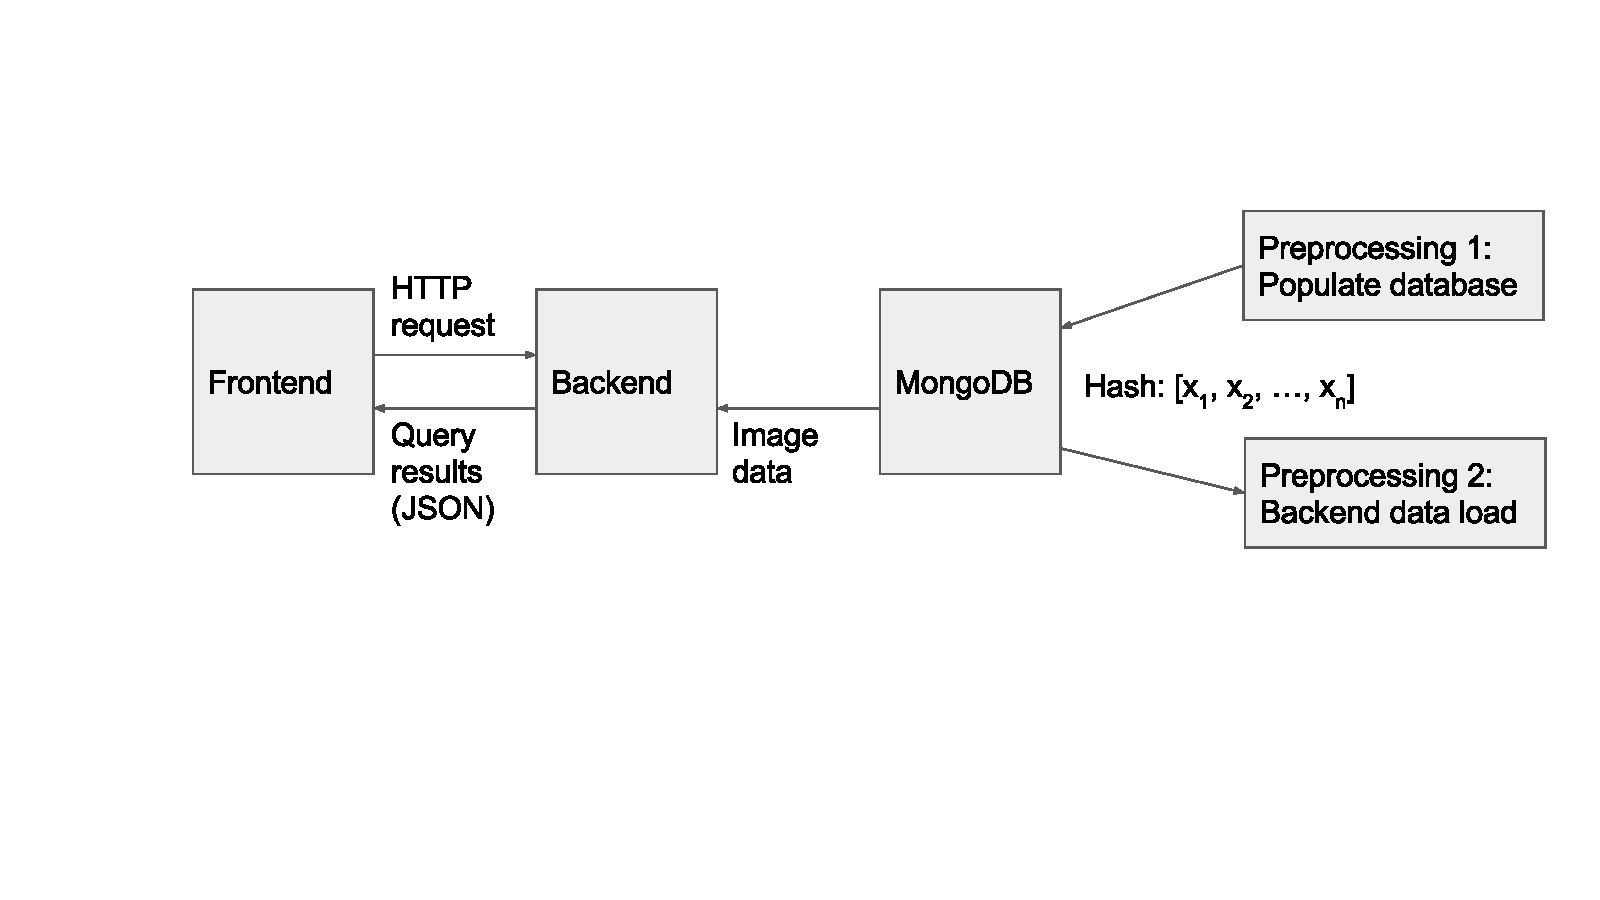
\includegraphics[width=0.9\columnwidth]{figs/system-design}
    \label{system-design}
\end{minipage}
The system works as follows:\\
    1. The frontend sends a series of query images (include and/or exclude) to the backend. \\
    2. The backend calculates the cosine distance from the hash of every query image to the hash of every image in the database.
    3. The backend then hands off these distances to post-processing where the algorithms mentioned in Section \ref{sec:algo}

\subsection{Frontend Design}
The frontend is implemented using Meteor~\cite{coleman2015discover} (special thanks to Michael Kaminsky).
The frontend allows users to see their entire image collection and select images to use as positive
and negative queries by clicking on them.

\subsection{Backend Design}
The backend is implemented in Python and accepts HTTP requests from the frontend.
The backend is persistent and uses a request-based model, rather than invoked upon every new user query,
which is done for performance reasons.
The main mechanism to calculate cosine distances between image hashes is to use the cdist function in the
scipy~\cite{jones2001open} library for Python.

Further work includes optimizing this calculation, as it is currently implemented not as matrix multiplication
but as for loops.
The reason for this seems to be to minimize floating point error, but an application such as this is very
tolerant to rounding and quantization, so we believe there are further performance gains possible on this
operation.

\subsection{Optimizations}
One of the goals of the system was to enable fast (<1s) queries of the image set in order to achieve
a good user experience.
In order to reach this performance goal, we implemented 2 preprocessing steps.
The first preprocessing step uses TensorFlow~\cite{abadi2016tensorflow} to generate hashes for each image and
store them in MongoDB.
The hash in this implementation of imagematch is the output of the pool\_3 layer of the Inception
model~\cite{szegedy2015going} pretrained on the 2012 ImageNet dataset.
Due to time constraints, using other layers was not explored in depth in this project and is left for
future work.
One possible difficulty in using the output of earlier layers is that the amount of memory and computation
increases as the size of the hash increases, and the activations output by earlier layers are larger than
the output of pool\_3.
This preprocessing step takes about TODO hours of CPU time to preprocess 300,000 images.

The second preprocessing step pre-loads all of the hashes from MongoDB into a matrix stored by the backend.
This allows queries to occur without any of the overhead associated with marshalling data into different formats.
This step takes about TODO 120 seconds to complete and is done once every time the dataset changes.

\section{Evaluation}
The evaluation of the query result quality and the performance were done completely separately.
The former was done using user studies and on a hand-picked image set (dataset 1), while the latter was done
on an arbitrarily chosen subset of the ImageNet dataset\cite{krizhevsky2012imagenet} (dataset 2).

Dataset 1 is of modest size (about 150 images), whereas dataset 2 varies in size from 10,000 to 300,000 images.
Due to time constraints, image sets larger than 300,000 images were left for future work.

\section{Summary}
